\section{Определение расширенной комплексной плоскости. Описать алгоритм
построения сферы Римана. Сделать поясняющий
рисунок.}\label{ux43eux43fux440ux435ux434ux435ux43bux435ux43dux438ux435-ux440ux430ux441ux448ux438ux440ux435ux43dux43dux43eux439-ux43aux43eux43cux43fux43bux435ux43aux441ux43dux43eux439-ux43fux43bux43eux441ux43aux43eux441ux442ux438.-ux43eux43fux438ux441ux430ux442ux44c-ux430ux43bux433ux43eux440ux438ux442ux43c-ux43fux43eux441ux442ux440ux43eux435ux43dux438ux44f-ux441ux444ux435ux440ux44b-ux440ux438ux43cux430ux43dux430.-ux441ux434ux435ux43bux430ux442ux44c-ux43fux43eux44fux441ux43dux44fux44eux449ux438ux439-ux440ux438ux441ux443ux43dux43eux43a.}

\textbf{Определение:} Комплексная плоскость, дополненная бесконечно
удаленной точкой, называется \emph{расширенной комплексной плоскостью} и
обозначается \(\overline{\mathbb{C}}\), т.е. \[
\overline{\mathbb{C}}=\mathbb{C}\cup \{ \infty \}
\]

\subsubsection{Построение сферы Римана (стереографическая
проекция)}\label{ux43fux43eux441ux442ux440ux43eux435ux43dux438ux435-ux441ux444ux435ux440ux44b-ux440ux438ux43cux430ux43dux430-ux441ux442ux435ux440ux435ux43eux433ux440ux430ux444ux438ux447ux435ux441ux43aux430ux44f-ux43fux440ux43eux435ux43aux446ux438ux44f}

\begin{enumerate}
\def\labelenumi{\arabic{enumi}.}
\tightlist
\item
  Берём сферу \(S\), касающуюся комплексной плоскости \(\mathbb{C}\) в
  точке \(O\) (точка касания совпадает с началом координат).
\item
  Обозначаем через \(P\) точку сферы, диаметрально противоположную точке
  касания \(O\) (верхняя точка сферы).
\item
  Каждой точке \(z \in \mathbb{C}\) ставим в соответствие точку \(M\)
  --- точку пересечения сферы \(S\) с отрезком, соединяющим \(z\) и
  \(P\).
\item
  Это соответствие \(z \leftrightarrow M\) между точками плоскости и
  точками сферы (кроме \(P\)) взаимно однозначно.
\item
  Единственная точка сферы, не имеющая прообраза на плоскости, --- сам
  полюс \(P\). Последовательности \(\{z_n\}\) с \(|z_n| \to \infty\)
  соответствует последовательность точек сферы, сходящаяся к \(P\).
  Поэтому точке \(z = \infty\) ставят в соответствие \(P\).
\end{enumerate}

\subsubsection{Формулы стереографической проекции
(опционально)}\label{ux444ux43eux440ux43cux443ux43bux44b-ux441ux442ux435ux440ux435ux43eux433ux440ux430ux444ux438ux447ux435ux441ux43aux43eux439-ux43fux440ux43eux435ux43aux446ux438ux438-ux43eux43fux446ux438ux43eux43dux430ux43bux44cux43dux43e}

Введём координаты: плоскость \(\mathbb{C}\) --- это плоскость
\(\{w = 0\}\) в пространстве \((u, v, w)\), где точке \(z = x + iy\)
отвечает \((x, y, 0)\). Сферу \(S\), касающуюся плоскости в точке \(O\),
зададим уравнением

\[u^2 + v^2 + \left(w - \tfrac12\right)^2 = \tfrac14\]

(радиус \(\tfrac12\), нижняя точка --- \(O = (0,0,0)\), полюс ---
\(P = (0,0,1)\)).

Тогда соответствие \(z \leftrightarrow M\) из алгоритма выписывается в
координатах явно. Точке \(z\) отвечает точка \(M = (u, v, w)\) сферы:

\[u = \frac{x}{1+|z|^2}, \quad v = \frac{y}{1+|z|^2}, \quad w = \frac{|z|^2}{1+|z|^2};\]

обратно, по точке \(M\) восстанавливается \(z\):

\[x = \frac{u}{1-w}, \quad y = \frac{v}{1-w}.\]

Эти формулы делают взаимную однозначность соответствия
\(z \leftrightarrow M\) явной. При \(|z| \to \infty\) получаем
\(w \to 1\), то есть точка \(M\) стремится к полюсу \(P\) --- что
согласуется с сопоставлением \(z = \infty \leftrightarrow P\) из пункта
5.

\textbf{Определение:} соответствие между точками расширенной комплексной
плоскости \(\overline{\mathbb{C}} = \mathbb{C} \cup \{\infty\}\) и
точками сферы \(S\) взаимно однозначно. Сфера \(S\) с таким
соответствием называется \textbf{сферой Римана}.

\pandocbounded{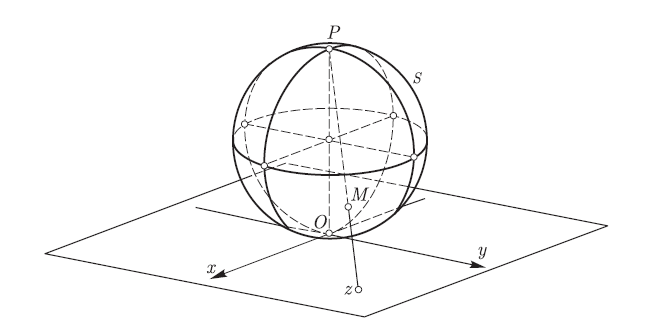
\includegraphics[keepaspectratio]{Вопросы/media/Pasted image 20260605161528.png}}
